\item \points{36} {\bf Neural Networks: MNIST image classification}

In this problem, you will implement a simple neural network
to classify grayscale images of handwritten digits (0 - 9) from
the MNIST dataset. The dataset contains 60,000 training images and
10,000 testing images of handwritten digits, 0 - 9. Each image is
28$\times$28 pixels in size, and is generally represented as a flat
vector of 784 numbers. It also includes labels for each example, a number
indicating the actual digit (0 - 9) handwritten in that image. A sample of
a few such images are shown below.

\begin{center}
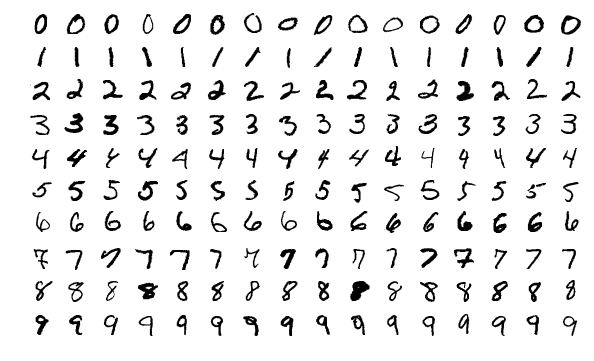
\includegraphics[scale=0.5]{mnist/mnist_plot}
\end{center}

The data and starter code for this problem can be found in

\begin{itemize}
\item \texttt{src/mnist/nn.py}
\item \texttt{src/mnist/images\_train.csv}
\item \texttt{src/mnist/labels\_train.csv}
\item \texttt{src/mnist/images\_test.csv}
\item \texttt{src/mnist/labels\_test.csv}
\end{itemize}

The starter code splits the set
of 60,000 training images and labels into a set of 50,000 examples as
the training set, and 10,000 examples for dev set.

To start, you will implement a neural network with a single hidden layer
and cross entropy loss, and train it with the provided data set. You will use the
sigmoid function as activation for the hidden layer and use the cross-entropy loss for multi-class classification. Recall that for a single example $(x, y)$, the cross
entropy loss is:
%\tnote{change the notation here to make it more consistent with the lecture }
$$\ell_\textup{CE}(\bar{h}_{\theta}(x),y) = - \log\left(\frac{\exp(\bar{h}_{\theta}(x)_{y})}{\sum_{s=1}^{k}\exp({\bar{h}_{\theta}(x)}_s)}\right),$$
where $\bar{h}_{\theta}(x) \in \mathbb{R}^{k}$ is the logits, i.e., the output of the the model on a training example $x$, $\bar{h}_\theta(x)_y$ is the $y$-th coordinate of the vector $\bar{h}_\theta(x)$ (recall that $y\in \{1,\dots, k\}$ and thus can serve as an index.)

%\tnote{let's call the one-hot vector $e_y$ so that we don't have to overload the notation. Can still keep the $\hat{y}$. The cross-entropy loss should be defined the same as in the lecture notes}


We have labeled data $(x^{(i)}, y^{(i)})_{i=1}^n$, where $x^{(i)} \in \mathbb{R}^d$, and $y^{(i)} \in \{1,\dots, k\}$ is ground truth label. Note that, in this specific application, we pass in the \textit{flattened} images as input. In other words, if each original input image is in $\mathbb{R}^{r \times r}$, we have $x^{(i)} \in \mathbb{R}^{r^2}$.

Additionally, let $m$ be the number of hidden units in the neural network, so that weight matrices $W^{[1]} \in \mathbb{R}^{d \times m}$ and $W^{[2]} \in \mathbb{R}^{m \times k}$.\footnote{Please note that the dimension of the weight matrices is different from those in the lecture notes, but we also multiply ${W^{[1]}}^\top$ instead of $W^{[1]}$ in the matrix multiplication layer.  Such a change of notation is mostly for some consistence with the convention in the code.} We also have biases $b^{[1]} \in \mathbb{R}^m$ and $b^{[2]} \in \mathbb{R}^k$. The parameters of the model $\theta$ is $(W^{[1]},W^{[2]},b^{[1]},b^{[2]})$.

We define the following neural network with a single hidden layer, which we refer to as the \textbf{Linear Layer NN}. For a single input $x^{(i)}$, the forward propagation equations are:

\begin{align}
  a^{(i)} &= \sigma \left( {W^{[1]}}^\top x^{(i)}  + b^{[1]} \right)  \in \mathbb{R}^m \nonumber \\
  \bar{h}_{\theta}(x^{(i)})&= {W^{[2]}}^\top a^{(i)} + b^{[2]} \in \mathbb{R}^k \nonumber \\
  {h}_{\theta}(x^{(i)}) &=  \mathrm{softmax}(\bar{h}_{\theta}(x^{(i)})) \in \mathbb{R}^k \nonumber
\end{align}
where $\sigma$ is the sigmoid function. 

For $\nexp$ training examples, we average the cross entropy loss over the $\nexp$ examples.
  \begin{equation*}
  J(W^{[1]},W^{[2]},b^{[1]},b^{[2]}) = \frac{1}{\nexp}\sum_{i=1}^\nexp \ell_\textup{CE}(\bar{h}_{\theta}(x^{(i)}),y^{(i)})  = - \frac{1}{\nexp}\sum_{i=1}^\nexp \log\left(\frac{\exp(\bar{h}_{\theta}(x^{(i)})_{y^{(i)}})}{\sum_{s=1}^{k}\exp({\bar{h}_{\theta}(x^{(i)})}_s)}\right).
  \end{equation*}

Suppose $e_y\in \Re^k$ is the one-hot embedding/representation of the discrete label $y$, where the $y$-th entry is 1 and all other entries are zeros. We can also write the loss function in the following way:
  \begin{equation*}
  J(W^{[1]},W^{[2]},b^{[1]},b^{[2]}) = - \frac{1}{\nexp}\sum_{i=1}^\nexp e_{\ysi}^\top\log\left(h_\theta(x^{(i)})\right).
  \end{equation*}
Here $\log(\cdot)$ is applied entry-wise to the vector $h_\theta(\xsi)$. The starter code already converts labels into one-hot representations for you.


Instead of batch gradient descent or stochastic gradient descent, the common practice
is to use mini-batch gradient descent for deep learning tasks. Concretely, we randomly sample $B$ examples $(x^{(i_k)}, y^{(i_k)})_{k=1}^B$ from $(x^{(i)}, y^{(i)})_{i=1}^n$. In this case, the
mini-batch cost function with batch-size $B$ is defined as follows:

  \begin{equation*}
  J_{MB} = \frac{1}{B}\sum_{k=1}^B \ell_\textup{CE}(\bar{h}_{\theta}(x^{(i_k)}),y^{(i_k)})
  \end{equation*}
where $B$ is the batch size, i.e., the number of training examples in each mini-batch.

\begin{enumerate}
  \item \points{5} 

%For a single input example $x^{(i)}$ with one-hot label vector $y^{(i)}$, show that $$\nabla_{z^{(i)}} \mathrm{CE}(y^{(i)}, \hat{y}^{(i)}) = \nabla_{z^{(i)}} \mathrm{CE}(y^{(i)}, \mathrm{softmax}(z^{(i)}) ) = \hat{y}^{(i)} - y^{(i)} \in \mathbb{R}^K$$


%\tnote{Tengyu's edit starts}


Let $t\in \R^k, y\in \{1,\dots, k\}$ and $p = \softmax(t)$. 
Prove that 
\begin{align}
\frac{\partial \ell_\textup{CE}(t, y)}{\partial t} = p - e_y \in \Re^k,
\end{align}

where $e_y\in \Re^k$ is the one-hot embedding of $y$, (where the $y$-th entry is 1 and all other entries are zeros.)
As a direct consequence, 

\begin{align}
\frac{\partial \ell_\textup{CE}(\bar{h}_{\theta}(x^{(i)}), y^{(i)})}{\partial \bar{h}_{\theta}(x^{(i)})} = \mathrm{softmax}(\bar{h}_{\theta}(x^{(i)})) - e_{y^{(i)}}  = {h}_{\theta}(x^{(i)})- e_{y^{(i)}}\in \Re^k
\end{align}



%\tnote{Tengyu's edit ends}

%\tnote{use the above notation system, check the equation's correctness, and update the hints (or even maybe not hints? No hints sounds good to me)}




where $\bar{h}_{\theta}(x^{(i)}) \in \mathbb{R}^k$ is the input to the softmax function, i.e. $${h}_{\theta}(x^{(i)}) = \mathrm{softmax}(\bar{h}_{\theta}(x^{(i)}))$$

(Note: in deep learning, $\bar{h}_{\theta}(x^{(i)})$ is sometimes referred to as the "logits".)

%\textbf{Hint:} To simplify your answer, it might be convenient to denote the true label of $x^{(i)}$ as $l \in \{1,\dots,K\}$. Hence $l$ is the index such that that $y^{(i)} = [0,...,0,1,0,...,0]^\top$ contains a single 1 at the $l$-th position. You may also wish to compute $\displaystyle \frac{\partial \mathrm{CE}(y^{(i)}, \hat{y}^{(i)})}{\partial z^{(i)}_j}$ for $j\neq l$ and $j=l$ separately.


\ifnum\solutions=1 {
  \begin{answer}
\end{answer}
   
  

} \fi

  \item \points{15} 

%\tnote{to update math notations below. }
%\tnote{double check consistenty with code. Ideally we should make minimal changes to the code}

Implement both forward-propagation and back-propagation for the above loss function $J_{MB} = \frac{1}{B}\sum_{k=1}^B \ell_\textup{CE}(\bar{h}_{\theta}(x^{(i_k)}),y^{(i_k)})
$.
Initialize the weights of the network by sampling values from a standard normal
distribution. Initialize the bias/intercept term to 0.
Set the number of hidden units to be 300, and learning rate to be 5. Set $B = 1,000$
(mini batch size). This means that we train with 1,000 examples in each iteration.
Therefore, for each epoch, we need 50 iterations to cover the entire training data.
The images are pre-shuffled. So you don't need to randomly sample the data, and can
just create mini-batches sequentially.


Train the model with mini-batch gradient descent
as described above. Run the training for 30 epochs. At the end of each epoch, calculate
the value of loss function averaged over the entire training set, and plot it
(y-axis) against the number of epochs (x-axis). In the same image, plot the value
of the loss function averaged over the dev set, and plot it against the number of epochs.

Similarly, in a new image, plot the accuracy (on y-axis) over the training set,
measured as the fraction of correctly classified examples, versus the number of epochs
(x-axis). In the same image, also plot the accuracy over the dev set versus number of epochs.

\textbf{Submit the two plots (one for loss vs epoch, another for accuracy vs epoch) in your writeup.}

Also, at the end of 30 epochs, save the learnt parameters (i.e., all the weights and biases)
into a file, so that next time you can directly initialize the parameters with
these values from the file, rather than re-training all over. You do NOT need to
submit these parameters.


\textbf{Hint:} Be sure to vectorize your code as much as possible! Training can be
very slow otherwise. For better vectorization, use one-hot label encodings in the code ($e_y$ in part (a)).


\ifnum\solutions=1 {
  \begin{answer}
\end{answer}
   
  

} \fi

  \item \points{7} Now add a regularization term to your cross entropy loss.
The loss function will become \begin{equation*}
  J_{MB} = \left(\frac{1}{B}\sum_{k=1}^B \ell_\textup{CE}(\bar{h}_{\theta}(x^{(i_k)}),y^{(i_k)})\right)
 + \lambda \left(||W^{[1]}||^2 + ||W^{[2]}||^2 \right)
  \end{equation*}
Be careful not to regularize the bias/intercept term.
Set $\lambda$ to be 0.0001. Implement the regularized version and plot the same
figures as part (a). Be careful NOT to include the regularization term to measure
the loss value for plotting (i.e., regularization should only be used for gradient calculation for
the purpose of training).

\textbf{Submit the two new plots obtained with regularized training (i.e loss (without regularization term) vs epoch, and accuracy vs epoch) in your writeup.}

\textbf{Compare the plots obtained from the regularized model with the plots obtained
from the non-regularized model, and summarize your observations in a couple of sentences.}

As in the previous part, save the learnt parameters (weights and biases) into a
different file so that we can initialize from them next time.



\ifnum\solutions=1 {
  \begin{answer}
\end{answer}
   
  

} \fi


  \item \points{3}
All this while you should have stayed away from the test data completely. Now that
you have convinced yourself that the model is working as expected (i.e., the
observations you made in the previous part matches what you learnt in class
about regularization), it is finally time to measure the model performance on
the test set. Once we measure the test set performance, we report it (whatever
value it may be), and NOT go back and refine the model any further.

Initialize your model from the parameters saved in part (a) (i.e., the non-regularized
model), and evaluate the model performance on the test data. Repeat this using the
parameters saved in part (b) (i.e., the regularized model).

Report your test accuracy for both regularized model and non-regularized model.  
Briefly (in one sentence) explain why this outcome makes sense.
You should have accuracy close to 0.92870 without regularization, and 0.96760 with regularization.
Note: these accuracies assume you implement the code with the matrix dimensions as specified in
the comments, which is not the same way as specified in your code. Even if you do not precisely these
numbers, you should observe good accuracy and better test accuracy with regularization.
\ifnum\solutions=1 {
  \begin{answer}
\end{answer}
   
  

} \fi

  \item \points{6} In this part, we compare the model complexity of the Linear Layer NN model with a convolution-based model. Let the original input image be a grayscale image with height and width $r$, meaning each image is of shape (1, $r$, $r$).

We define a \textbf{CNN} (convolutional neural network) version of our original model. We let the number of output classes be $k$, and we have the following operations:

1. \textit{Convolutional Layer}: We define \( a(i) \) as the output of applying a 2D convolutional layer with 32 filters (with bias) of size \( 3 \times 3 \), padding 1, stride 1, and ReLU activation on an input image \( x^{(i)} \in \mathbb{R}^{1 \times r \times r}\). % \in \mathbb{R}^{h \times h} 

\[a_1^{(i)} = \mathrm{ReLU}(\mathrm{Conv2D}(x^{(i)}))\]

2. \textit{Flattening}: After applying the convolution, we flatten \( a_1^{(i)} \) into a vector.

\[a_2^{(i)} = \mathrm{Flatten}(a_1^{(i)}))\]

3. \textit{Linear Transformation}: We apply a linear transformation to the flattened vector, mapping it to $\mathbb{R}^k$
\[
\bar{h}_{\theta}(x^{(i)}) = {W^{[2]}}^\top a_2^{(i)} + b^{[2]}
\]

4. \textit{Softmax Output}: We apply the softmax activation to obtain our final output.
\[
{h}_{\theta}(x^{(i)}) = \mathrm{softmax}(\bar{h}_{\theta}(x^{(i)})) 
\]

\begin{enumerate}
    \item \subquestionpoints{1} In the CNN model, what are the dimensions of $a(i)$ right after the convolutional layer (before the flattening operation) in terms of $r$?

    \item \subquestionpoints{1} In the CNN model, how many parameters are there in terms of in terms of the input height/width $r$ and the number of output classes $k$? % How many are there in the MNIST example ($r=28, k=10$)?

    \item \subquestionpoints{1} In the Linear Layer NN model, how many parameters are there in terms of the input height/width $r$, the number of hidden units $m$, and the number of output classes $k$? % How many are there in the MNIST example ($r=28, m=300, k=10$)?

    \item \subquestionpoints{1} What is the maximum value of $m$ for which the Linear NN model has fewer parameters than the CNN model on the MNIST dataset ($r=28, k=10$)?
    
    \item \subquestionpoints{2} What is one advantage and one disadvantage of using the CNN compared to the Linear Layer NN?
    
\end{enumerate}
\ifnum\solutions=1 {
  \begin{answer}
\end{answer}
} \fi

 \end{enumerate}

